\subsection{OpenGL硬件加速性能瓶颈研究}

关于OpenGL硬件加速整个实现流程的性能瓶颈优化分析工作Matthias Trapp在它的文章OpenGL-Performance and Bottlenecks\cite{OpenGL-Performance}提出了一套基本理论分析原则,这套原则在OpenGL硬件加速优化方向上有着很好的指导意义。下面就简单介绍以下他对OpenGL性能优化提出的一些研究看法。

\subsubsection{性能瓶颈模型}

传统的软件优化都是在致力于找到软件程序的热点,即10\%的那部分代码却花费了整个软件执行的90\%的时间,然而如今的图形硬件加速都是将任务分配到渲染管线的一个个阶段中,而且这些阶段都是并行工作的,所以其中的数据流就会造成如图\ref{fig:Bottleneck}所示的瓶颈,试想A模块处理完数据后向B模块传递,然后B开始处理,此时A又可以开始处理新的数据,因为A和B对数据的处理速度不同,加上A到B数据传输也需要花费时间,这样A每次处理完多少数据再传递给B则会大大影响整个工作的完成时间。

\begin{figure}[H] 
  \centering
  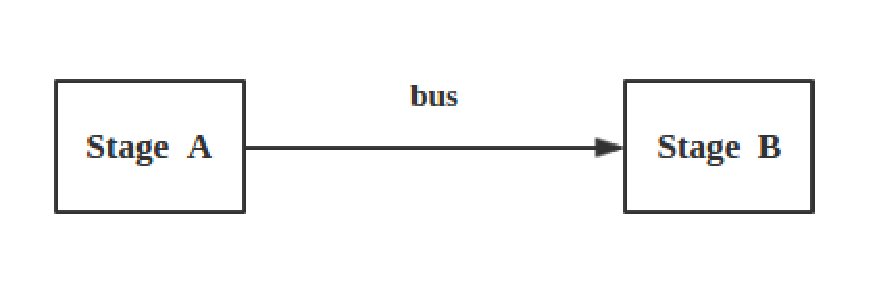
\includegraphics[width=5cm,height=2.5cm]{figures/chap02/Bottleneck-Model}
  \caption{OpenGL瓶颈模型}
  \label{fig:Bottleneck-Model}
\end{figure}

\subsubsection{性能瓶颈的分类}

从前面\ref{sec:Mesa3D-Flow}可以出OpenGL硬件加速主要有三个过程: CPU端计算、数据与命令传输、GPU渲染。所以大的方向来看这里面的性能瓶颈也可以分为以下三类:

\begin{itemize}
\item{\textbf{CPU计算瓶颈}}: 这部分很好理解,因为在硬件加速时候CPU端也需要做很多事情,而且是整个渲染流程的开端。这部分常见的性能瓶颈有很多,比如CPU向GPU每次发送数据规模较小,导致CPU计算时间占比较大,GPU闲死而CPU闲死。
\item{\textbf{CPU到GPU数据传输瓶颈}}: 这部分主要和数据传输效率有关,因为不同硬件环境下CPU和GPU的数据传输方式有很多,不同的方式传输带宽不同,这也会导致整个渲染流程阻塞。
\item{\textbf{GPU渲染瓶颈}}: 这部分主要和GPU硬件有关,不同的GPU环境也不一样,具体表现就是GPU无法很快的进行图形渲染。
\end{itemize}

\subsubsection{性能瓶颈的检测}

对于OpenGL性能瓶颈的检测,Matthias Trapp提出了两种方法:

\begin{itemize}
\item{}通过减少某一特定阶段的输入负载。通常从最早的阶段开始测试。如果整体性能有着较大提升,则说明此阶段为性能的瓶颈阶段。
\item{}通过减少其他阶段的负载量,甚至去掉其他阶段。如果整体性能并无多大变化,说明此阶段为性能的瓶颈阶段。
\end{itemize}

所以,我们可以通过这个方法来逐步检测前面提到的三类性能瓶颈问题从而确定瓶颈点,然后寻找解决办法。

\subsection{CPU与GPU数据传输的优化研究}

\subsubsection{CPU与GPU数据传输优化的通用研究}
当前GPU一般是通过PCI-E连接起来的进行数据传输的,而随着硬件设备的不断发展,GPU的计算性能提升速度远远快于PCI-E传输带宽的提升速度,所以CPU到GPU的数据传输就占据了很大一部分时间。为了尽量减少这段传输时间的占比,Sai Ma等人的文章Evaluate GPU performance with memory transfer overhead\cite{Evaluate-GPU}里面提出了三种解决办法: 异步内存操作、映射内存和CPU/GPU调度的优化。下面简单的对这集中方法做一点介绍。

\begin{itemize}
\item{\textbf{异步内存操作}} \\
由于很多GPU设备支持边拷贝边计算的能力,设备内核执行主机计算程序和主机到设备内存拷贝可以同时执行,这样就可以把数据传输和数执行划分为流水线步骤进行并发执行。如下图\ref{fig:Streaming}所示,将数据块划分为三块,然后形成三条流水线并行执行。
\\

\begin{figure}[H] 
  \centering
  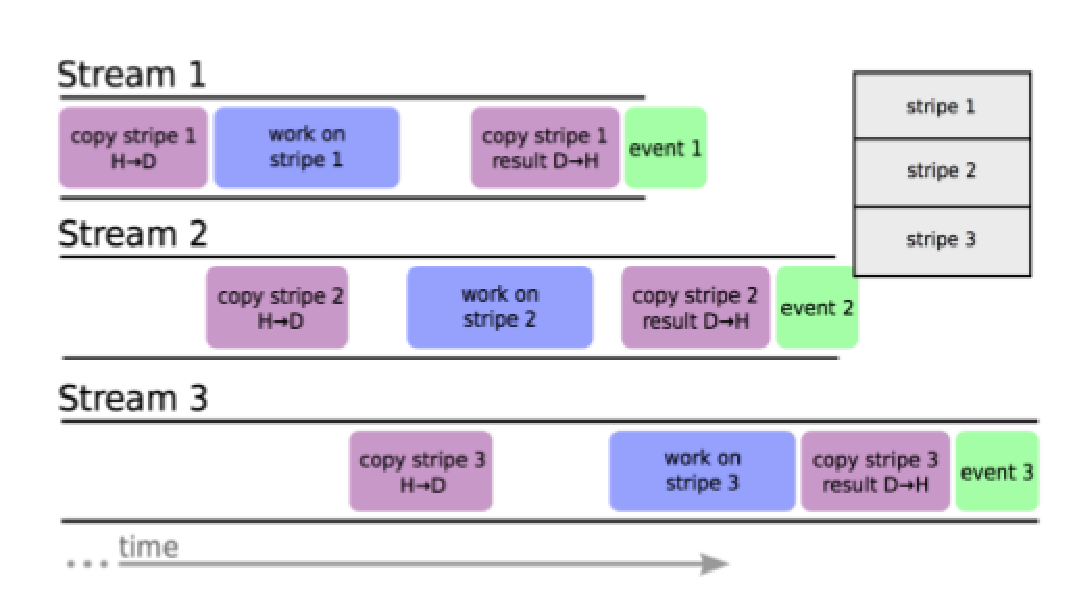
\includegraphics[width=5cm,height=2.5cm]{figures/chap02/Streaming}
  \caption{Streaming举例}
  \label{fig:Streaming}
\end{figure}
\item{\textbf{映射内存}} \\
通常来说GPU与CPU的组合方式分为两种,一种是独立CPU存在的,它们之间通过PCI-E线连接,传输速度较慢;而另外一种则是和CPU融合在一块的集成GPU,这样的GPU使用的内存就是CPU内存分配出去的一部分,所以这里面的拷贝则是CPU内存内部的拷贝,数据传输消耗就大大减少。当然集成GPU在计算性能方面可能不如独立GPU强大,而且这种优化方式实际上是硬件上的更换,可操作性不大。关于这两种GPU的更多比较可以查看参考文献On the Efficacy of a Fused CPU+GPU Processor(or APU) for Parallel Computing\cite{on-the-Efficacy}。
\\
\begin{figure}[H] 
  \centering
  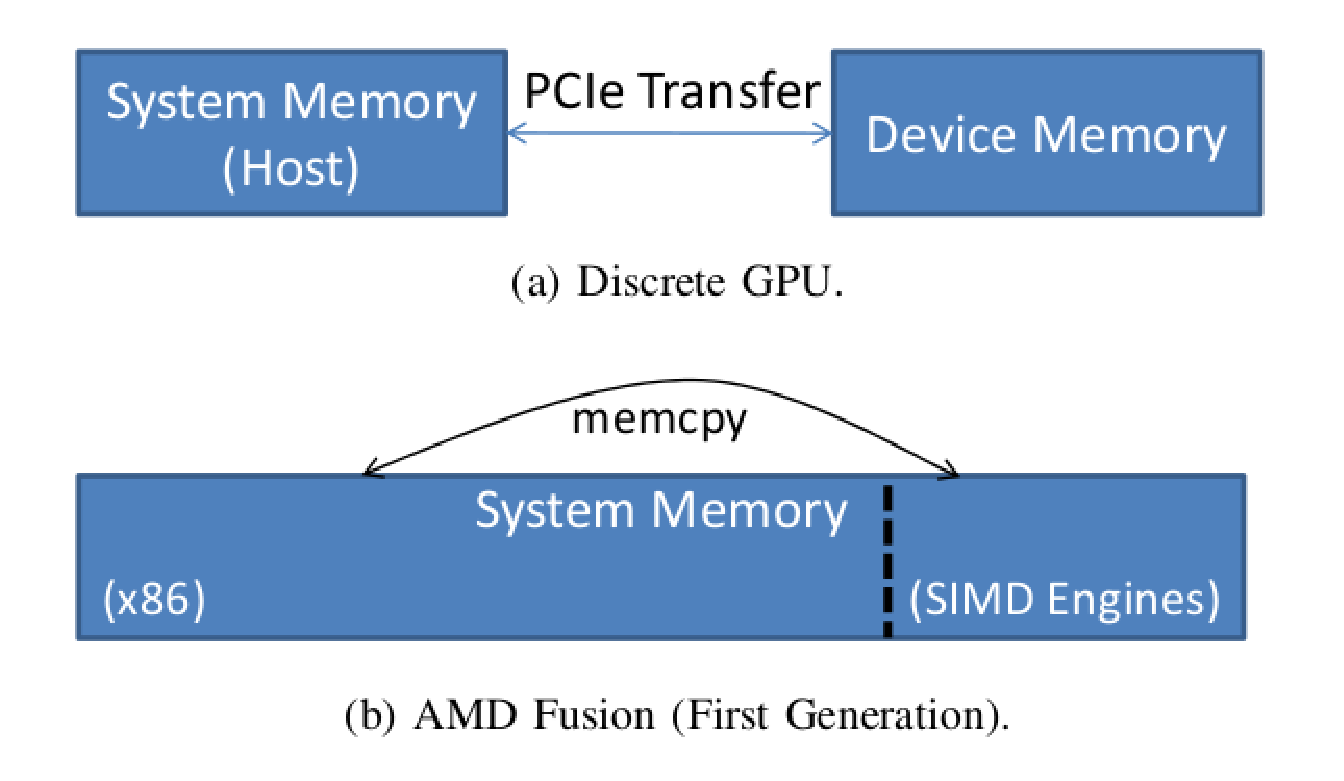
\includegraphics[width=5cm,height=2.5cm]{figures/chap02/Transfer}
  \caption{独立GPU与集成GPU的数据传输方式比较}
  \label{fig:Transfer}
\end{figure}
\item{\textbf{CPU/GPU调度的优化}} \\
这方面的优化简单来说就是重新修改应用程序,使得CPU的任务执行,GPU的任务执行以及CPU到GPU的数据传输之间次序做出一些调整。通过将任务和数据映射成任务数据关系图数学模型,然后再通过设定好最优解目标,使用模拟退火(Simulated Annealing)算法寻找最优任务与数据次序。
\end{itemize}

\subsubsection{龙芯平台上CPU与GPU数据传输的优化研究}

由于龙芯平台的特殊性,在龙芯平台上的CPU与GPU数据传输有着一些专门的优化方法,其中张凯在论文$<<$显存与内存间的数据传输通路优化$>>$\cite{gpu-cpu-data}里面提出了一种基于DMA的非线性传输优化。

我们以GPU端将数据从系统内存拷贝到显存为例,传统的实现方式有两种方法:

\begin{itemize}
\item{} GPU将系统主存地址空间通过GTT的方式映射到显存虚拟地址空间,然后就可以对其进行直接读写,这里面是通过PCI-E总线进行的读写。这种方式的优点就是实现简单,不过因为龙芯平台上PCI-E总线带宽较小,数据传输速率不高。
\item{} GPU通过DMA的方式将数据从系统主存拷贝到显存。当然,因为GPU并不能访问全部的系统内存,只能访问系统主存的GTT部分内存,所以这就需要先把数据拷贝到GTT中,然后再使用DMA方式进行数据的高速传输。这种方式实现比较复杂,不过传输效率较高。

通常来说,GPU对上面的两种方式都是支持的,而且在诸如X86平台上进行小数据的读写时候会采用第一种方式,因为DMA的方式需要一些额外的开销,更加适合大数据的传输。在龙芯平台上,由于PCI-E总线的传输效率很慢,成为瓶颈,所以在小数据时候DMA方式的读写效率也更高。
\end{itemize}
